\documentclass[mathserif,compress]{beamer}

\mode<presentation>
{
  \usecolortheme{}
  \definecolor{blue}{rgb}{0.8,0,0}
\setbeamercolor{ separation line }{bg=black}
  \setbeamercolor{frametitle}{bg=gray!20!white}
}
\newcommand\hmmax{0}
\newcommand\bmmax{0}
\usepackage{natbib, verbatim}

\usepackage[utf8]{inputenc}

\usepackage{mathpazo}
\usepackage[T1]{fontenc}

\usepackage{amsmath}
\usepackage{amsthm}
\usepackage{amssymb}
\usepackage{mathptmx}
\usepackage{anyfontsize}
\usepackage{t1enc}
\usepackage{appendix}
\usepackage{array}
\usepackage{bm}
\usepackage{cancel}
\usepackage[font=small,labelfont=bf]{caption}
\usepackage{cite}
\usepackage{courier}
\usepackage{graphicx}
\usepackage{empheq}
\usepackage{enumerate}
\usepackage{listings}
\usepackage{mathtools}
\usepackage{units}
\usepackage{bigstrut}
\usepackage{rotating}
\usepackage{ mathrsfs }
\usepackage{multirow}
\usepackage{booktabs}
\usepackage{algorithm, algorithmic}

\DeclareMathAlphabet{\mathcal}{OMS}{cmsy}{m}{n}

\DeclareMathAlphabet{\mathsfit}{\encodingdefault}{\sfdefault}{m}{}
\SetMathAlphabet{\mathsfit}{bold}{\encodingdefault}{\sfdefault}{bx}{}

\newcommand{\tens}[1]{\bm{\mathsfit{#1}}}

\usepackage{color}
\lstset{language=R,basicstyle=\ttfamily,breaklines=true,
                keywordstyle=\color{blue}\ttfamily,
                stringstyle=\color{red}\ttfamily,
                commentstyle=\color{magenta}\ttfamily,
                showstringspaces=false,
                }

\newcommand*\widefbox[1]{\fbox{\hspace{2em}#1\hspace{2em}}}
\newcommand*\mb{\mathbf}
\newcommand*\reals{\mathbb{R}}
\newcommand*\complex{\mathbb{C}}
\newcommand*\naturals{\mathbb{N}}
\newcommand*\nats{\naturals}
\newcommand*\integers{\mathbb{Z}}
\newcommand*\rationals{\mathbb{Q}}
\newcommand*\irrationals{\mathbb{J}}
\newcommand*\pd{\partial}
\newcommand*\htab{\hspace{4 mm}}
\newcommand*\vtab{\vspace{0.5 in}}
\newcommand*\lsent{\mathcal{L}}
\newcommand*\conj{\overline}
\newcommand*\union{\cup}
\newcommand*\intersect{\cap}
\newcommand*\cl{\cancel}
\newcommand*\ANS{\text{ANS}}
\newcommand*\As{\text{As}}
\newcommand*\then{\rightarrow}
\newcommand*\elim{\text{E}}
\newcommand*\intro{\text{I}}
\newcommand*\absurd{\curlywedge}
\newcommand*\NK{\vdash_{\text{NK}}}
\newcommand*\derivation{\begin{tabular} { >{$}l<{$}  >{$}c<{$}  >{$}l<{$}  >{$}r<{$} }}
\newcommand*\interp{\mathcal{I}}
\newcommand*\ba{\[ \begin{aligned}}
\newcommand*\ea{\end{aligned} \]}
\newcommand*\C{\mathcal{C}}
\newcommand*\D{\mathscr{D}}
\newcommand*\e{\operatorname{e}}
\newcommand*\df{=_{\text{def}}}
\newcommand*\eps{\epsilon}
\newcommand*\enum{\begin{enumerate}[label=(\alph*)]}
\newcommand*\enumend{\end{enumerate}}
\newcommand*\E[1]{\tens{E}\left[#1\right]}
\newcommand*\Esub[2]{\tens{E}_{#1}\left[#2\right]}
\newcommand*\Var[1]{\tens{Var}\left[#1\right]}
\newcommand*\Cov[1]{\tens{Cov}\left[#1\right]}
\newcommand*\iid{\overset{\text{iid}}{\sim}}
\newcommand*\Exp[1][\lambda]{\text{Exp}(\text{rate}=#1)}
\newcommand*\ind[1]{\mathbb{1}\left(#1\right)}
\newcommand*\set[1]{\left\{#1\right\}}
\newcommand*\estim[1]{\widehat{#1}}
\newcommand*\der{\text{d}}
\newcommand*\norm[1]{\left\|#1\right\|}
\newcommand*\dist[2]{\;\text{dist}\left(#1, #2\right)}
\newcommand*\interior{\text{int}\;}
\newcommand*\exterior{\text{ext}\;}
\newcommand*\boundary{\text{bd}\;}
\newcommand*\lh{\overset{\text{L'H}}{=}}

\renewcommand\Re{\operatorname{Re}}
\renewcommand\Im{\operatorname{Im}}
\DeclareMathOperator*{\argmin}{arg\;min}
\renewcommand\;{\,}
\renewcommand\epsilon{\varepsilon}
\renewcommand\rho{\varrho}
\renewcommand\phi{\varphi}
\renewcommand\mod{\hspace{0.2em} \textbf{mod}\hspace{0.2em}}
\renewcommand\Pr[1]{ \estim{\mathsf{Pr}}\left(#1\right) }
\def\ci{\perp\!\!\!\perp}

\usepackage{tikz}
\usetikzlibrary{positioning}
\usetikzlibrary{shapes,arrows}
\usepackage{adjustbox}

\tikzstyle{decision} = [diamond, draw, fill=blue!20, 
    text width=4.5em, text badly centered, node distance=3cm, inner sep=0pt]
\tikzstyle{block} = [rectangle, draw, fill=blue!20, 
    text width=6em, text centered, rounded corners, minimum height=4em]
\tikzstyle{line} = [draw, -latex']
\tikzstyle{cloud} = [draw, ellipse,fill=red!20, node distance=3cm,
    minimum height=2em]

\lstset{breaklines=true,
        numbersep=5pt,
        xleftmargin=.25in,
        xrightmargin=.25in}

\DeclareMathOperator{\sech}{sech}
\DeclareMathOperator{\sgn}{sgn}
\makeatletter
\renewcommand*\env@matrix[1][*\c@MaxMatrixCols c]{%
  \hskip -\arraycolsep
  \let\@ifnextchar\new@ifnextchar
  \array{#1}}
\makeatother

\newenvironment{amatrix}[1]{%
  \left(\begin{array}{@{}*{#1}{c}|c@{}}
}{%
  \end{array}\right)
}

\lstset{basicstyle=\footnotesize\ttfamily,breaklines=true}


\newcommand{\real}{\ensuremath{\mathbb{R}}}
\newcommand{\bA}{\mbox{\protect\boldmath $A$}}
\newcommand{\bo}{\mbox{\protect\boldmath $o$}}
\newcommand{\bu}{\mbox{\protect\boldmath $u$}}
\newcommand{\by}{\mbox{\protect\boldmath $y$}}
\newcommand{\bx}{\mathbf{x}}
\newcommand{\bs}{\mbox{\protect\boldmath $s$}}
\newcommand{\bS}{\mbox{\protect\boldmath $S$}}
\newcommand{\bz}{\mathbf{z}}
\newcommand{\bh}{\mbox{\protect\boldmath $h$}}
\newcommand{\bF}{\mbox{\protect\boldmath $f$}}
\newcommand{\bt}{\mbox{\protect\boldmath $t$}}
\newcommand{\bc}{\mbox{\protect\boldmath $c$}}
\newcommand{\bC}{\mbox{\protect\boldmath $C$}}
\newcommand{\bp}{\mbox{\protect\boldmath $p$}}
\newcommand{\bV}{\mbox{\protect\boldmath $V$}}
\newcommand{\bX}{\mbox{\protect\boldmath $X$}}
\newcommand{\bW}{\mbox{\protect\boldmath $W$}}
\newcommand{\bZ}{\mbox{\protect\boldmath $Z$}}
\newcommand{\bof}{\mbox{\protect\boldmath $f$}}
\newcommand{\indicator}{{\ensuremath{\mathbb{I}}}}
\newcommand{\M}{{\ensuremath{\rm M}}}
\newcommand{\bbeta}{\boldsymbol{\beta}}
\newcommand{\balpha}{\boldsymbol{\alpha}}
\newcommand{\bgamma}{\boldsymbol{\gamma}}
\newcommand{\bdelta}{\boldsymbol{\delta}}
\newcommand{\bmu}{\boldsymbol{\mu}}
\newcommand{\bSigma}{\boldsymbol{\Sigma}}
\newcommand{\btheta}{\protect\boldsymbol{\theta}}
\newcommand{\bzero}{\mathbf{0}}
\newcommand{\hsp}{\hspace{0.2mm}}

\footnotesize

\beamertemplatenavigationsymbolsempty
\setbeamertemplate{headline}{\vskip2pt}

\title[]{Combining Mixture Components for Clustering}

\author[]
{Jean-Patrick Baudry, Adrian E. Raftery, Gilles Celeux, Kenneth Lo, and Rapha$\ddot{\text e}$l Gottardo\\$\;$ \\Presented by Branden Olson}

\date[April, 2018]
{April 12, 2018}

\institute[]
{
}

%Prepare a short presentation based on your chosen paper (10 slides at most). The main points you need to cover are:
%
%1. What is the scientific problem your paper is considering?
%
%2. What has been done to solve this problem before (aka literature review)?
%
%3. What new ideas do the authors propose?
%
%4. What are the interesting findings of the experiments on real data?

\begin{document}

\begin{frame}[noframenumbering]
  \titlepage
\end{frame}

\begin{frame}\frametitle{Scientific Problem}
\begin{itemize}
\item
Goal: Given data $X_1, \dotsc, X_n \in \reals^d$, form \alert{clusters} of similar groups
\begin{center}
\includegraphics[width=0.8\linewidth]{clustered.pdf}
\end{center}
\item
Problems:
\medskip
\begin{enumerate}
\item
Underlying distribution unknown
\medskip
\item
Number \& structure of clusters often unknown
\end{enumerate}
\end{itemize}
\end{frame}

\begin{frame}\frametitle{Previous work}
\begin{itemize}
\item
Clustering: very broad 
\medskip
\item
Our focus: model-based clustering
\medskip
\item
Assume $\bx_i \sim$ \alert{multivariate normal mixture}:
\ba
f(\bx_i ; K, \theta_K) 
	& = \sum_{k=1}^K p_k
		\phi \left(\bx_i ; \mu_k, \Sigma_k\right)
\ea
\smallskip
\item
Given $K$, get MLE 
$\estim\theta_K = (\mathbf p, \pmb\mu, \pmb\Sigma)$ using EM algorithm
\medskip
\item
Assign cluster labels based on MAP estimates
\medskip
\item
Goals: \alert{Select $K$} among candidates $\set{K_\text{min}, \dotsc, K_\text{max}}$,  \& \alert{infer cluster structure}
\medskip
\end{itemize}
\end{frame}

\begin{frame}\frametitle{Previous work}
\begin{itemize}
\item
Dasgupta \& Raftery (1998): $\estim K = \argmin_K \text{BIC}(K)$, where
\ba
\text{BIC}(K)
	= \underbrace{\log \; f(\bx; K, \estim\theta_K)}_\text{\alert{observed} log-likelihood} 
	- \frac{\nu_K \log(n)}{2}
\ea
\begin{itemize}
\item
Good for \# mixture components, bad for \# clusters
\end{itemize}
\medskip
\item
Biernacki et al. (2000): $\estim K = \argmin_K \text{ICL}(K)$, where
\ba
\text{ICL}(K)
	= \underbrace{\log \; f(\bx, \text{\color<1>[rgb]{0,0.7,0}{$\estim\bz$}}; K, \estim\theta_K)}_\text{\alert{"completed"} log-likelihood} - \frac{\nu_K \log(n)}{2}
\ea
\begin{itemize}
\item
Penalizes entropy of clustering
\medskip
\item
Treats non-Gaussian clusters as Gaussian
\end{itemize}
\end{itemize}
\end{frame}

\begin{frame}\frametitle{New ideas}
\begin{itemize}
\item
Exploit respective strengths of BIC and ICL:
\begin{enumerate}
\medskip
\item
Use BIC to choose \# mixture components
\medskip
\item
Sequentially merge clusters to minimize overall entropy
\medskip
\item
Yields \alert{sequence of clusterings} for $K_\text{min}, \dotsc, K_\text{max}$
\medskip
\item
Choose $K$ substantially or when entropy "levels out"
\end{enumerate} 
\bigskip
\item
Allows (\# components) $\ne$ (\# clusters)
\bigskip
\item
Maximizes likelihood \& minimizes entropy
\bigskip
\item
Complexity: $\mathcal O \left( \left\{\text{rate for } \estim K_\text{BIC} \right\}+ n K_\text{max}^3 \right)$
\end{itemize}
\end{frame}

\begin{frame}\frametitle{Illustration}
\begin{itemize}
\item
Simulate from 6-component mixture, and cluster:
\medskip
\begin{center}
\begin{minipage}{0.32\linewidth}
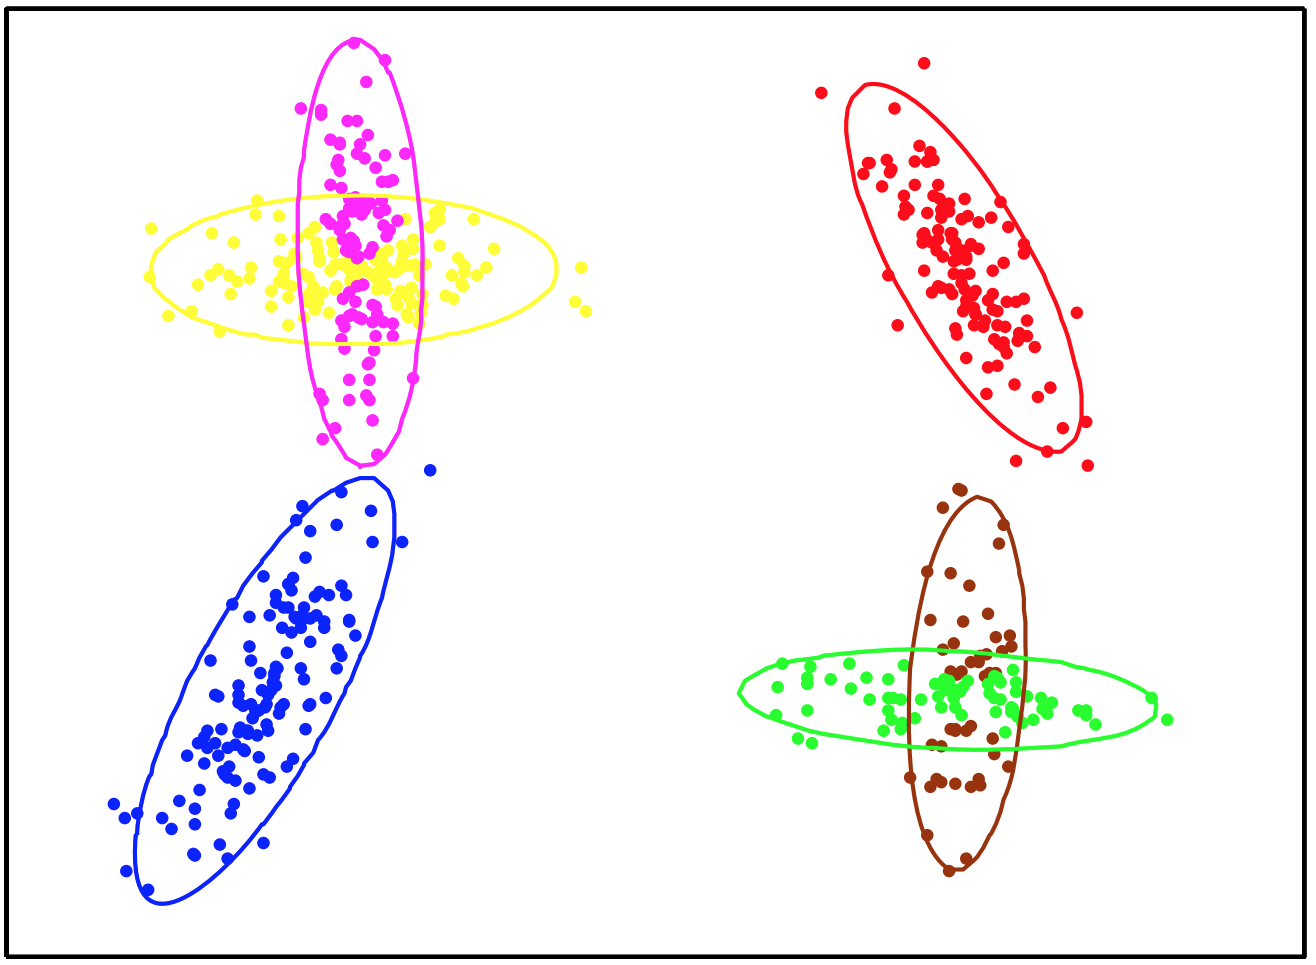
\includegraphics[width=\linewidth]{BIC.png}
\begin{center}
BIC solution
\end{center}
\end{minipage}
\hfill
\begin{minipage}{0.32\linewidth}
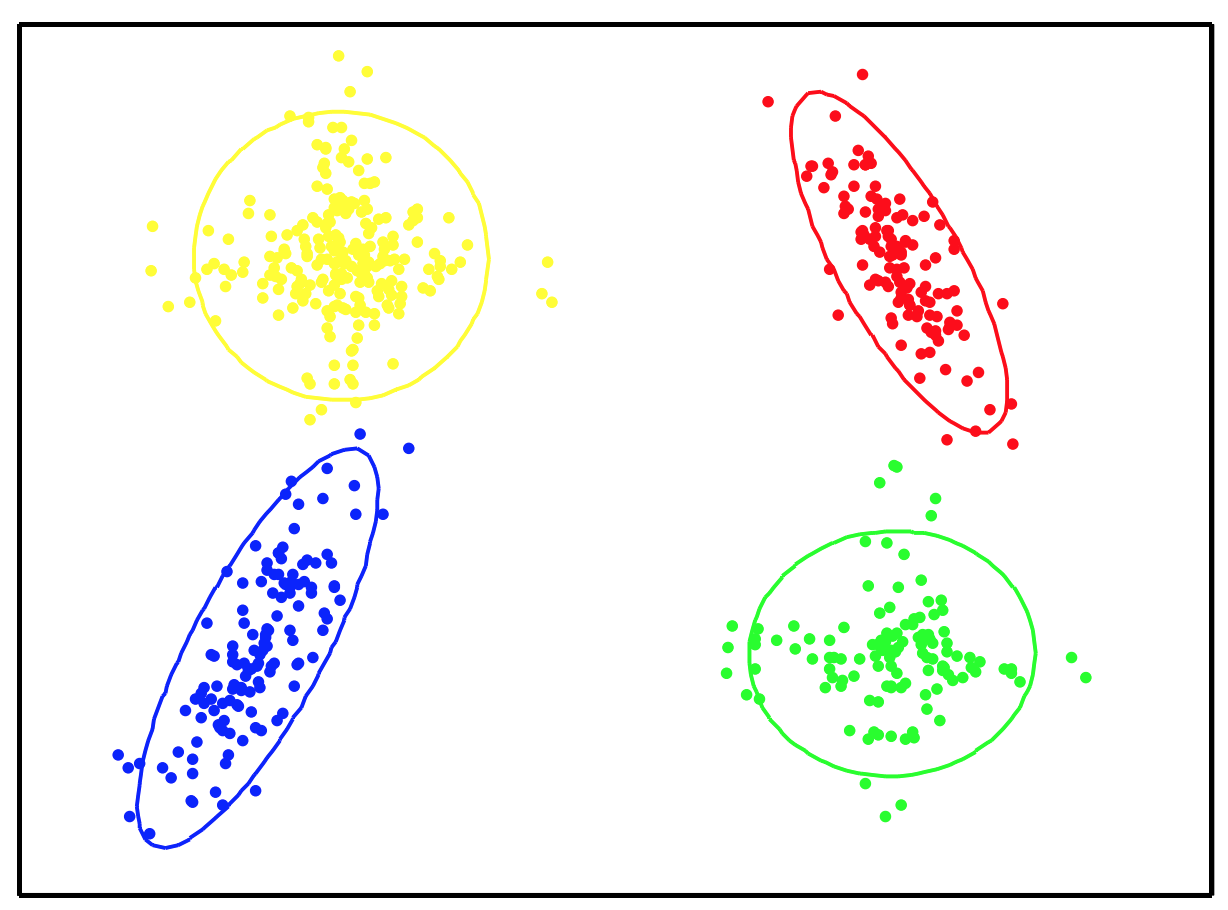
\includegraphics[width=\linewidth]{ICL.png}
\begin{center}
ICL solution
\end{center}
\end{minipage}
\hfill
\begin{minipage}{0.32\linewidth}
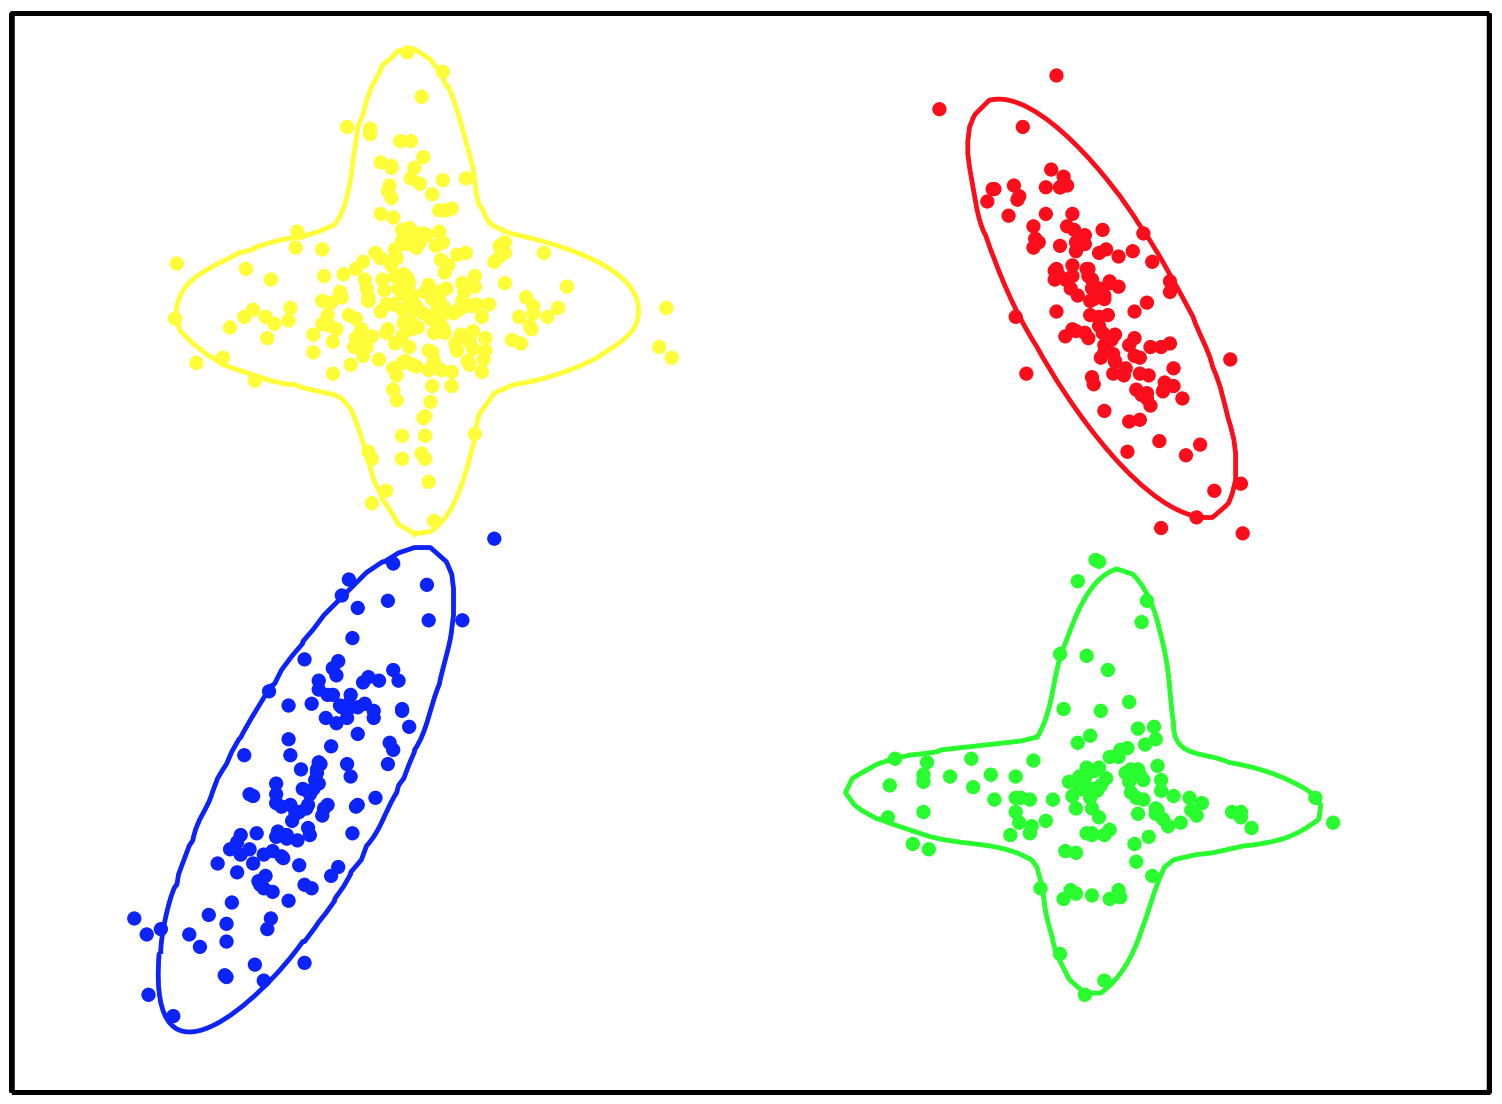
\includegraphics[width=\linewidth]{Combined.png}
\begin{center}
Combined solution
\end{center}
\end{minipage}
\end{center}
\bigskip
\item
Yields well-separated clusters like ICL
\medskip
\item
Can approximate non-Gaussian clusters as Gaussian mixtures
\end{itemize}
\end{frame}

\begin{frame}\frametitle{Case study: Flow cytometry data (Brinkman et al. 2007)}
\begin{itemize}
\item
Data: Biomarkers (protein molecules) from patients with \& without graft-vs-host disease 
\bigskip
\item
Goal: Identify cell sub-populations positive in 3 particular biomarkers (CD3$^+$CD4$^+$CD8$\beta^+$ cells) of the 4 collected
\bigskip
\item
Assume Gaussian mixture model with general $\Sigma_k$
\bigskip
\item
Cluster using BIC, ICL, \& 'combined' (Baudry et al.)
\end{itemize}
\end{frame}

\begin{frame}\frametitle{Experiments}
\begin{center}
\includegraphics[width=0.8\linewidth]{positive.pdf}
\end{center}
\end{frame}

\begin{frame}\frametitle{Experiments}
\begin{center}
\includegraphics[width=0.75\linewidth]{control.pdf}
\end{center}
\end{frame}

\begin{frame}\frametitle{Discussion}
\begin{itemize}
\item
BIC estimates components well for good model fit
\medskip
\item
ICL identifies clusters well for good model interpretation
\medskip
\item
Key idea: Allow $\left(\# \text{ mixture components}\right)$ 
$\ne$ 
$\left(\# \text{ clusters} \right)$ for good fit \& interpretation
\medskip
\item
Evidence of superior performance on real data 
\end{itemize}
\medskip
References:
\\
\medskip
\tiny
(1)
Biernacki, C., Celeux, G., and Govaert, G. (2000), ``Assessing a Mixture Model for Clustering With the Integrated
Completed Likelihood,'' IEEE Transactions on Pattern Analysis and Machine Intelligence, 22, 719?725.
\\ \smallskip
(2) Brinkman, R. R. et al. (2007), ``High-Content Flow Cytometry and Temporal Data Analysis for Defining a Cellular Signature of
Graft-versus-Host Disease,'' Biology of Blood and Marrow Transplantation, 13, 691?700.
\\ \smallskip
(3) Dasgupta, A., and Raftery, A. E. (1998), ``Detecting Features in Spatial Point Processes With Clutter via ModelBased
Clustering,'' Journal of the American Statistical Association, 93, 294?302. 
\end{frame}

\end{document}























